% Created 2019-02-06 Wed 20:36
% Intended LaTeX compiler: pdflatex
\documentclass[11pt]{article}
\usepackage[utf8]{inputenc}
\usepackage{lmodern}
\usepackage[T1]{fontenc}
\usepackage{fixltx2e}
\usepackage{graphicx}
\usepackage{longtable}
\usepackage{float}
\usepackage{wrapfig}
\usepackage{rotating}
\usepackage[normalem]{ulem}
\usepackage{amsmath}
\usepackage{textcomp}
\usepackage{marvosym}
\usepackage{wasysym}
\usepackage{amssymb}
\usepackage{amsmath}
\usepackage[version=3]{mhchem}
\usepackage[numbers,super,sort&compress]{natbib}
\usepackage{natmove}
\usepackage{url}
\usepackage{minted}
\usepackage{underscore}
\usepackage[linktocpage,pdfstartview=FitH,colorlinks,
linkcolor=blue,anchorcolor=blue,
citecolor=blue,filecolor=blue,menucolor=blue,urlcolor=blue]{hyperref}
\usepackage{attachfile}
\author{Myrthe Boone}
\date{\today}
\title{}
\begin{document}



\section*{RMS TITANIC: Machine learning from disaster}
\label{sec:org1dce408}
Profielwerkstuk Wiskunde D  

7 februari 2019

Myrthe Boone 6E

\begin{figure}[htbp]
\centering
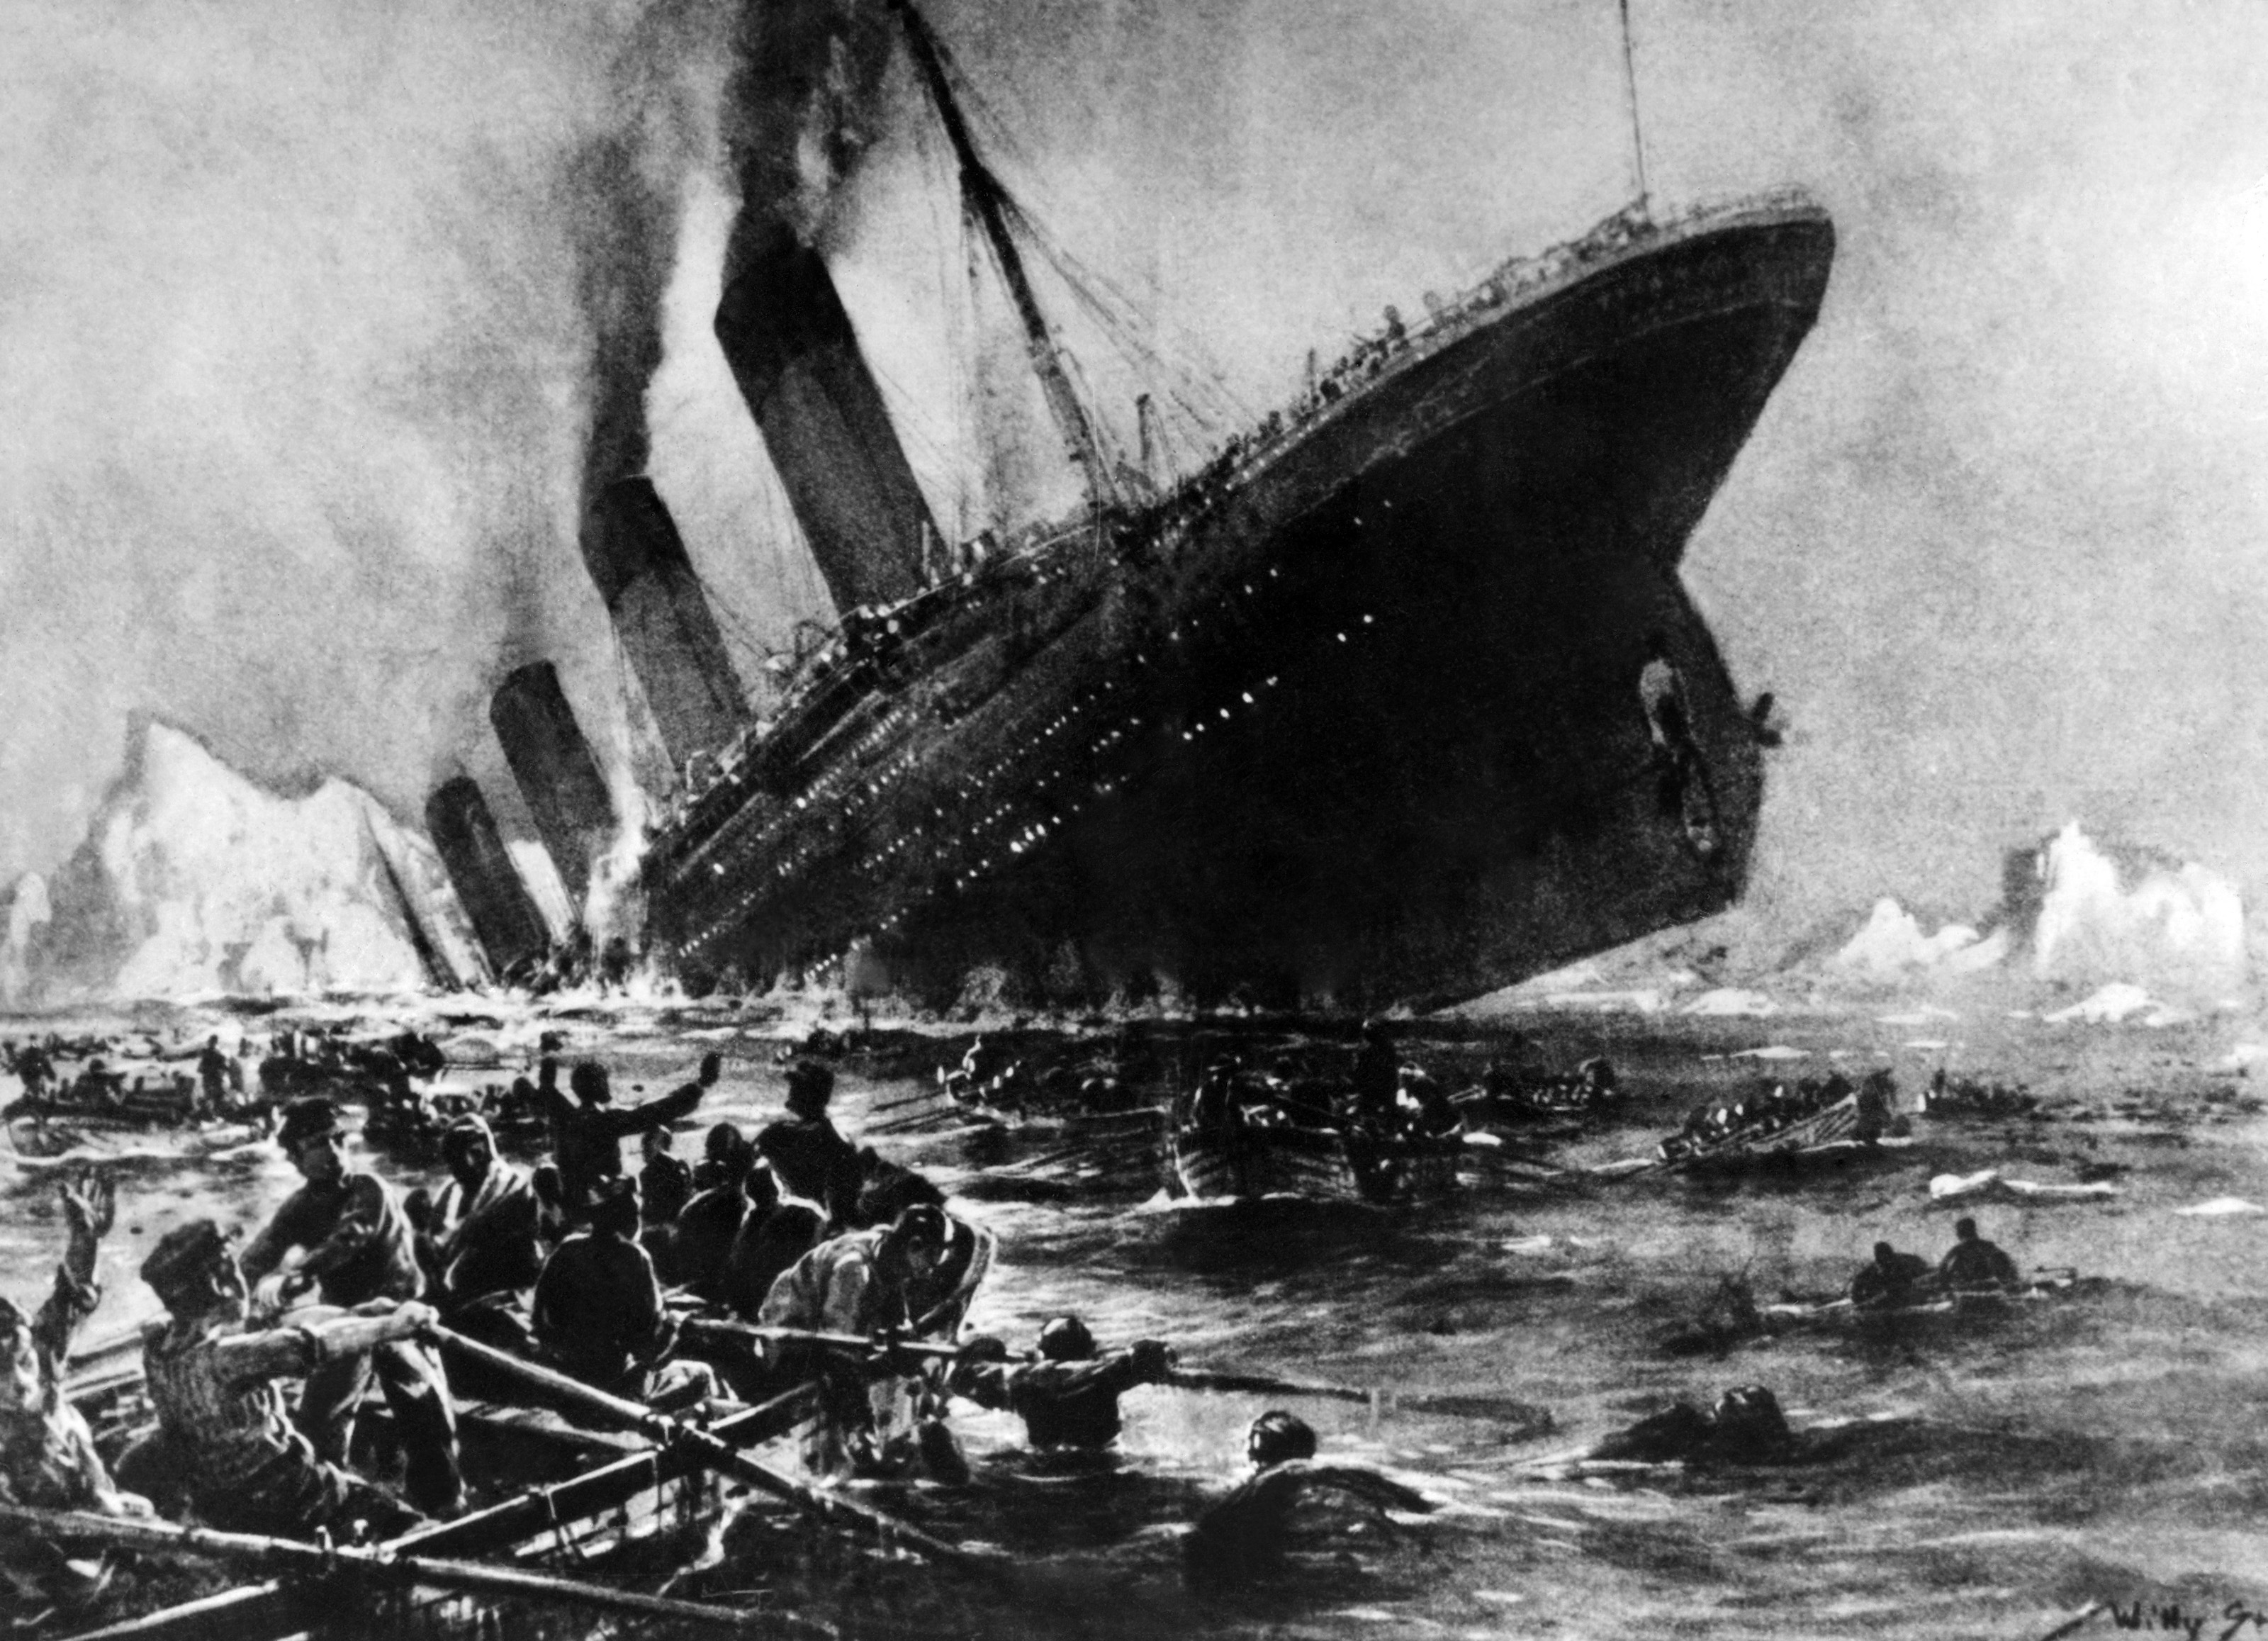
\includegraphics[width=.9\linewidth]{./Titanic.png}
\caption{RMS Titanic}
\end{figure}

\subsection*{Doodle}
\label{sec:org7b0b2c9}
\url{https://quickdraw.withgoogle.com/}

\section*{Inhoudsopgave}
\label{sec:orgccecb10}

\begin{itemize}
\item Introductie
\item Wat is machine learning?
\item Mijn onderzoek
\begin{itemize}
\item Algoritmes
\item Hoofd- en deelvragen
\end{itemize}
\item Resultaten
\item Conclusie
\item Discussie
\item Afsluiting
\end{itemize}

\section*{Introductie}
\label{sec:orgd9b3c78}
\subsection*{Waarom dit onderwerp?}
\label{sec:orge43ae05}

\begin{itemize}
\item Meer weten over machine learning en programmeren in Python
\item Machine learning is overal om ons heen
\item Organiseren en analyseren van de werkelijkheid
\item TU Eindhoven
\end{itemize}

\subsection*{Titanic}
\label{sec:orgb03a75f}

\begin{itemize}
\item Voorspellen welke groep passagiers een grotere kans had om te overleven.
\item 'Vrouwen en kinderen eerst' beleid
\item Geluk, geslacht, leeftijd, klasse en prijs betaald voor een ticket
\end{itemize}
\begin{figure}[htbp]
\centering
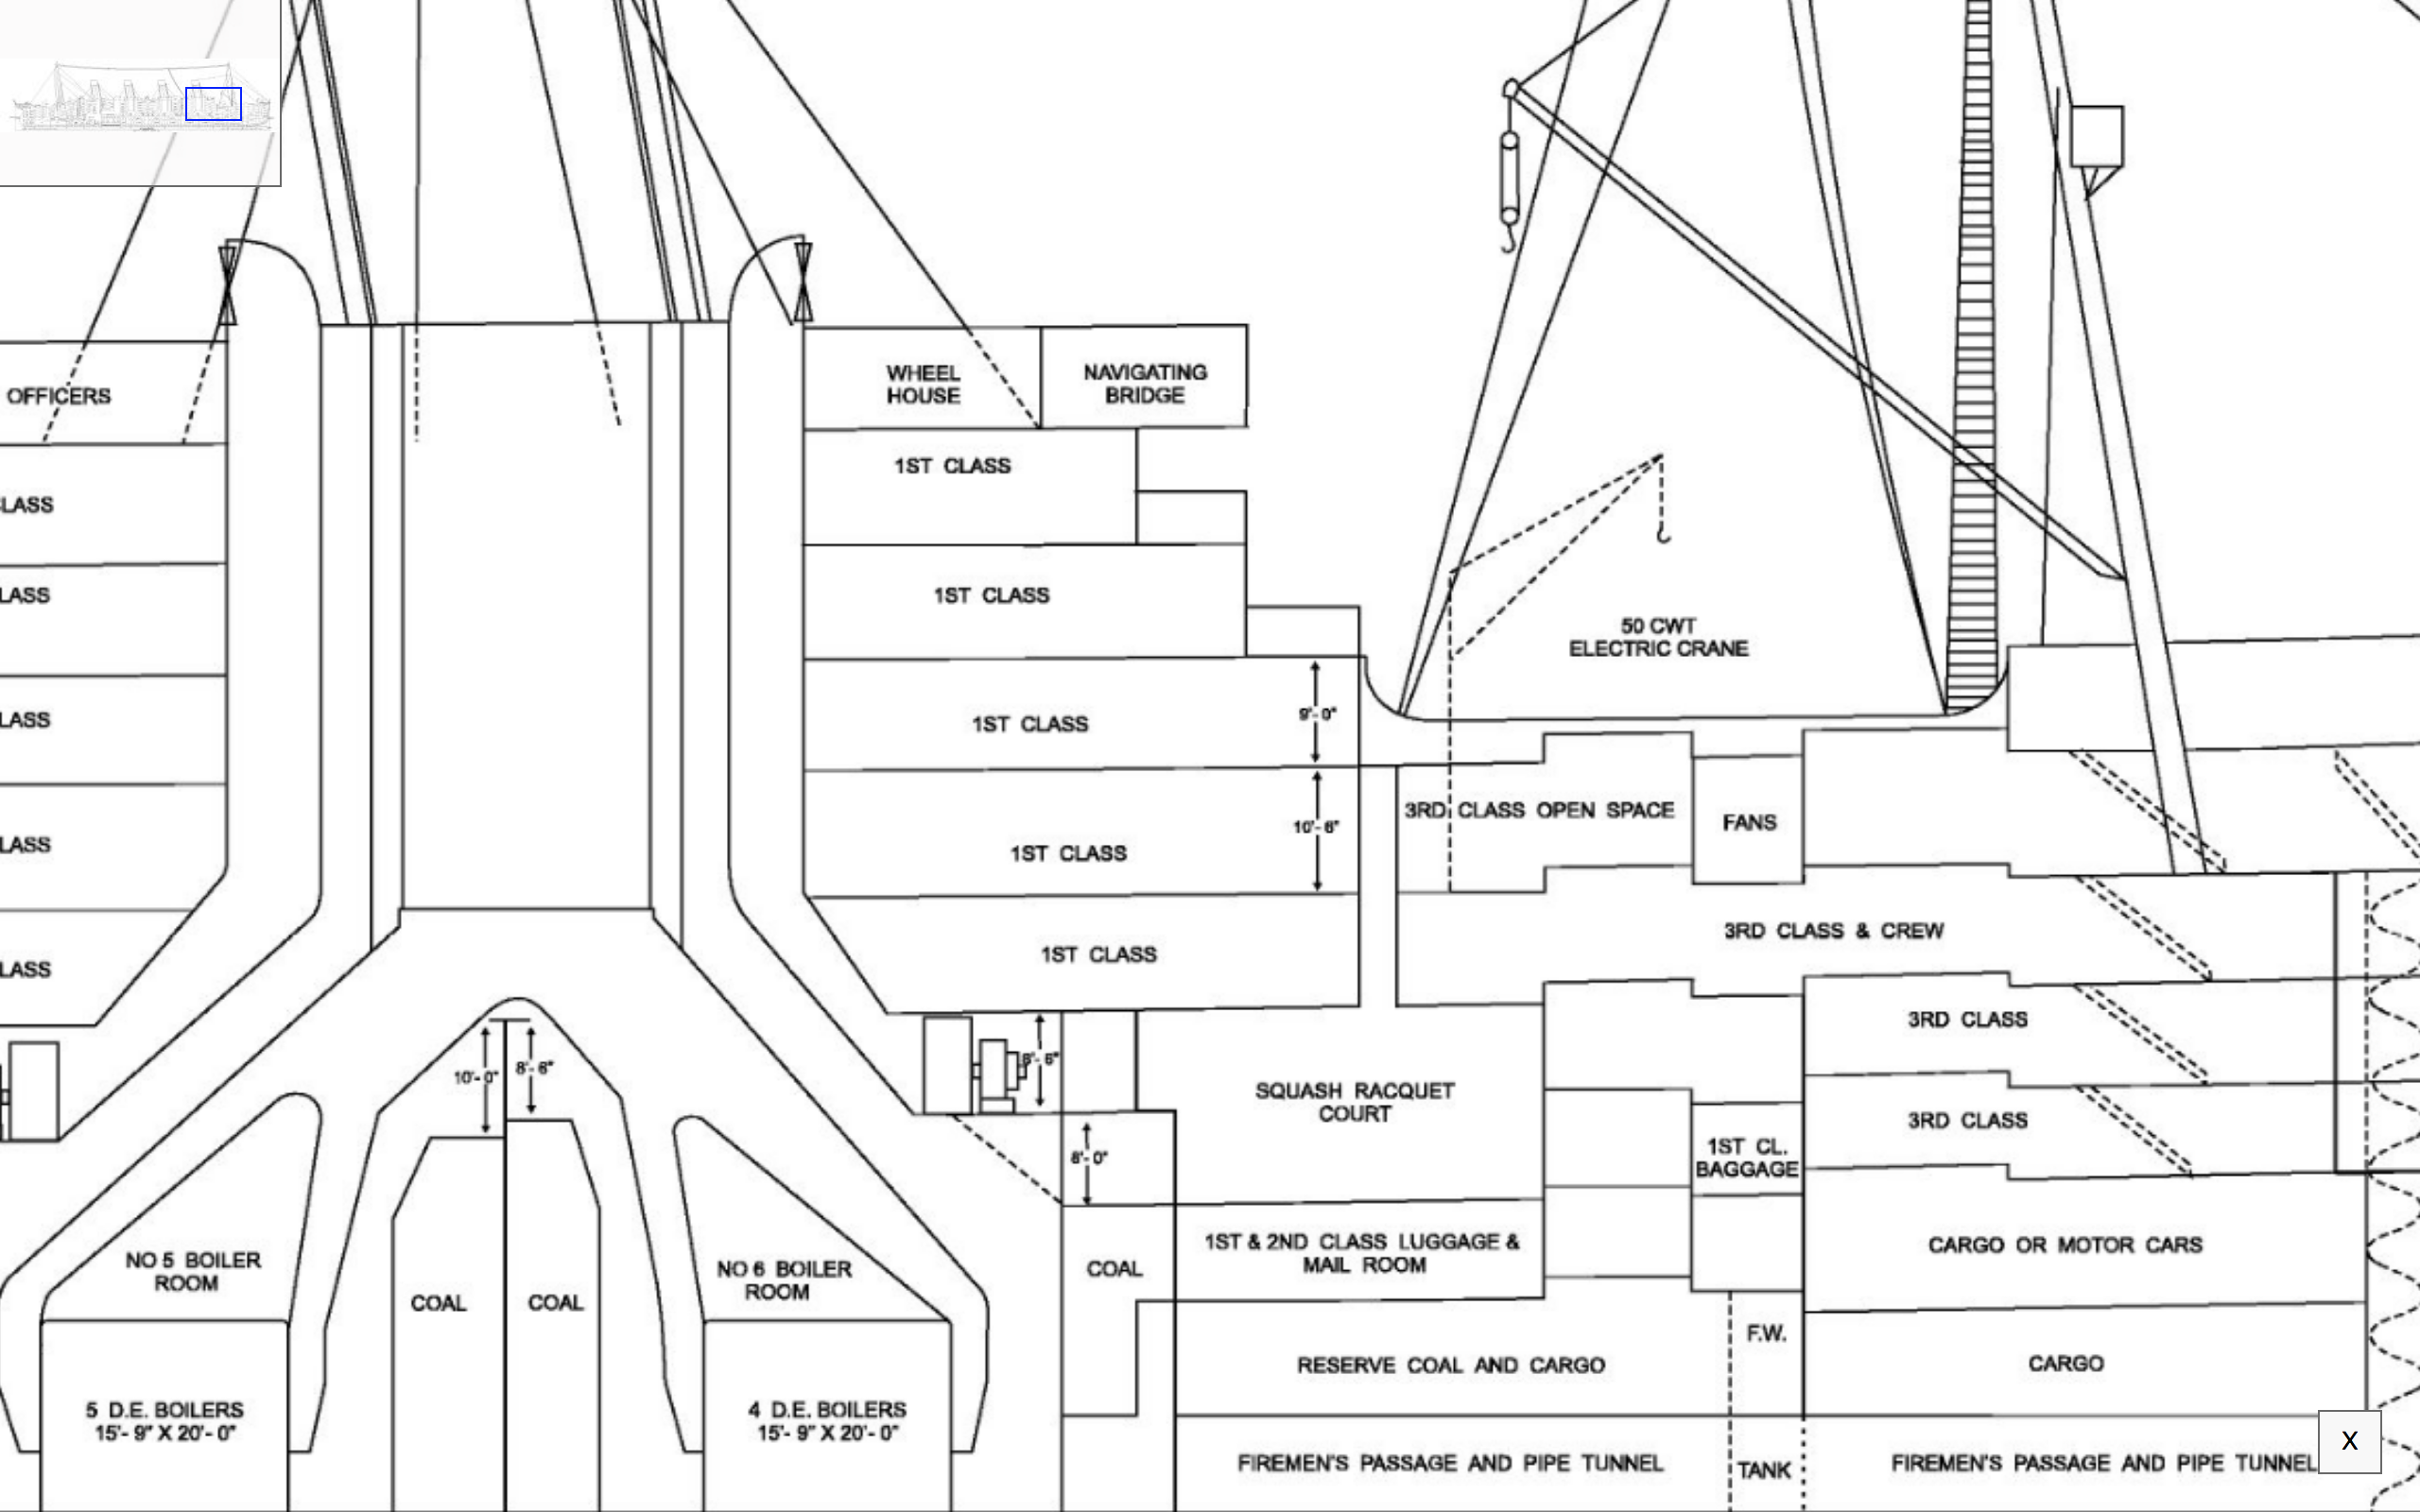
\includegraphics[width=600]{./Deck3.png}
\caption{\label{}
Deck Titanic}
\end{figure}


\section*{Wat is machine learning?}
\label{sec:org047cbfd}

\begin{itemize}
\item Zonder specifiek geprogrammeerd te zijn voor de taken
\item Voorbeeld: spam emails, Google zoekopdrachten
\end{itemize}

\begin{center}

\includegraphics[width=600]{./google.png}
\end{center}

\subsection*{Soorten machine learning}
\label{sec:orgf05f319}

\begin{itemize}
\item Supervised, unsupervised en reinforcement learning
\item Unsupervised: Correcte labels zijn \textbf{niet} gegeven
\item Supervised: Computer weet welke categorieën er zijn
\item Supervised learning kan ingedeeld worden in regression en classification
\end{itemize}

\begin{figure}[htbp]
\centering
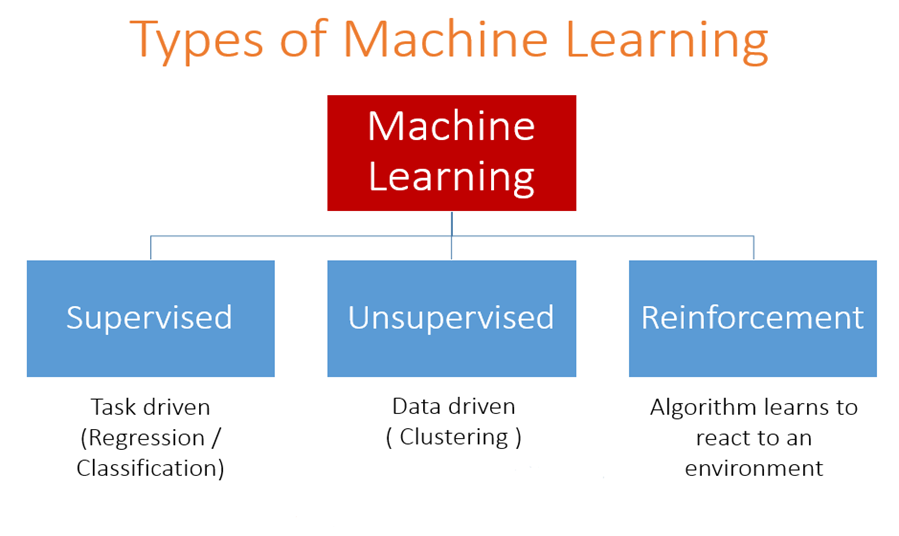
\includegraphics[width=600]{./typesmachinelearning.png}
\caption{Machine learning}
\end{figure}

\subsection*{Soorten machine learning}
\label{sec:org2d44d19}
\begin{itemize}
\item Classification: categorieën
\item Regression: continue variabelen
\end{itemize}
\begin{figure}[htbp]
\centering
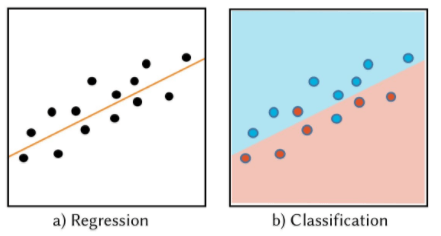
\includegraphics[width=600]{./regvsclass.png}
\caption{Classification vs. Regression}
\end{figure}


\subsection*{Soorten machine learning}
\label{sec:orge91a569}
\begin{itemize}
\item Titanic is supervised learning
\item Binary classification
\item 1 = overleefd
\item 0 = niet overleefd
\end{itemize}

\section*{Mijn onderzoek: algoritmes}
\label{sec:org4b67bf1}
\subsection*{Werkplan}
\label{sec:org3653e17}

\begin{itemize}
\item We splitsen onze dataset in een training en een test set
\item We trainen / fitten ons model op de training set
\item We voorspellen op de test set
\item Dus we gebruiken de gegevens van de passagiers (leeftijd, geslacht, prijs betaald voor een ticket, klasse)
\end{itemize}


\subsection*{Logistic Regression}
\label{sec:org9d59dc8}

\begin{itemize}
\item Gebaseerd op de logistische functie
\item Grenswaarde \(p>0.5\), passagier heeft het overleefd
\end{itemize}

\begin{equation}
\label{eq:2}
\sigma(y) = \frac{e^y}{1+e^y}
\end{equation}

\begin{itemize}
\item Vier variabelen dus \(y\) is in dit geval:
\end{itemize}

\begin{equation}
y=a_1x_1+a_2x_2+a_3x_3+a_4x_4+b+\varepsilon_{i} 
\end{equation}

\begin{figure}[htbp]
\centering
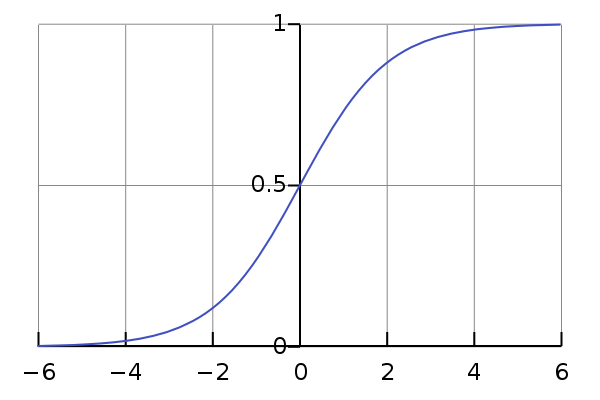
\includegraphics[width=600]{./LogisticCurve.png}
\caption{Logistische functie}
\end{figure}


\subsection*{Hoofd- en deelvragen}
\label{sec:orge6a1a1c}

\begin{itemize}
\item Is het mogelijk een nauwkeurige voorspelling te maken of de passagiers aan boord van de Titanic het hebben overleefd met behulp van informatie over geslacht, klasse, leeftijd en prijs betaald voor een ticket? 
\begin{itemize}
\item Wat is de invloed van geslacht op de overlevingskans?
\item Wat is de invloed van klasse op de overlevingskans?
\item Wat is de invloed van leeftijd op de overlevingskans?
\item Wat is de invloed van prijs betaald voor een ticket op de overlevingskans?
\end{itemize}
\end{itemize}

\section*{Resultaten}
\label{sec:orgaa1723a}
\subsection*{Dataset verkennen}
\label{sec:org0948277}

\begin{itemize}
\item Begonnen met plots maken, dataset ontdekken
\end{itemize}


\begin{figure}[htbp]
\centering
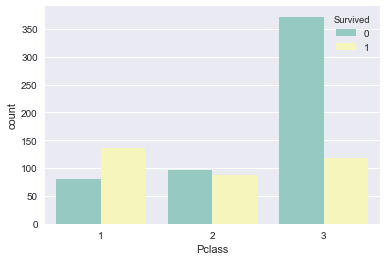
\includegraphics[width=600]{./ClassCount.png}
\caption{Plot van reisklasse}
\end{figure}

\subsection*{Resultaten}
\label{sec:orgc44b7c1}

\begin{itemize}
\item Coëfficiënten
\item Wat vertellen ze ons?
\end{itemize}

\subsection*{Resultaten}
\label{sec:org69dae9f}
\begin{itemize}
\item Coëfficiënt behorend bij leeftijd is negatief
\item Coëfficiënt behorend bij ticketprijs is positief
\item Geslacht coëfficiënt negatief (dummy)
\end{itemize}


\begin{figure}[htbp]
\centering

\includegraphics[width=600]{./coefficients.png}
\caption{}
\end{figure}

\begin{figure}[htbp]
\centering
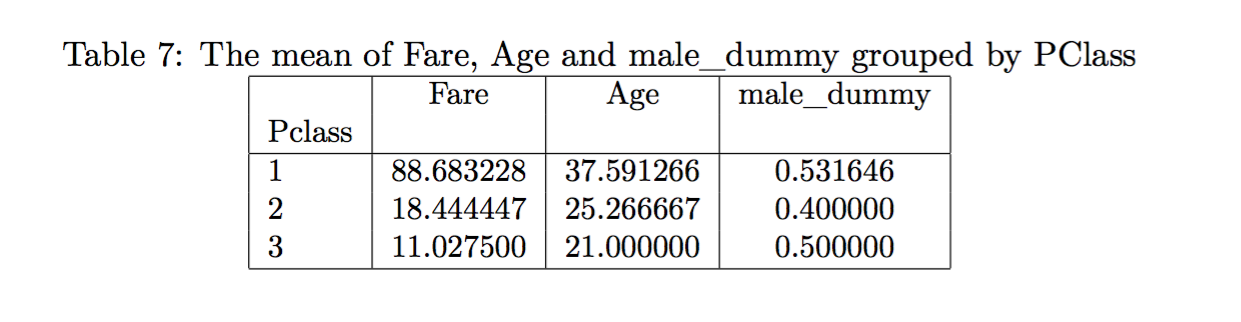
\includegraphics[width=600]{./Table7.png}
\caption{}
\end{figure}

\section*{Conclusie}
\label{sec:org3a799b0}

\begin{itemize}
\item Het is mogelijk een voorspelling te maken
\item Vrouwen hadden een voordeel t.o.v. mannen
\item Jongere passagiers hadden een voordeel t.o.v. oudere
\item Passagiers die een hogere ticketprijs hadden betaald hadden voordeel t.o.v. zij die minder betaalden
\end{itemize}



\section*{Discussie}
\label{sec:orgff7f7ea}
\begin{itemize}
\item Blijft een ongeluk: toeval, geluk, corruptie etc.
\item Meer variabelen
\item Nauwkeurigheid?
\item Invloed variabelen onderling
\end{itemize}


\begin{center}
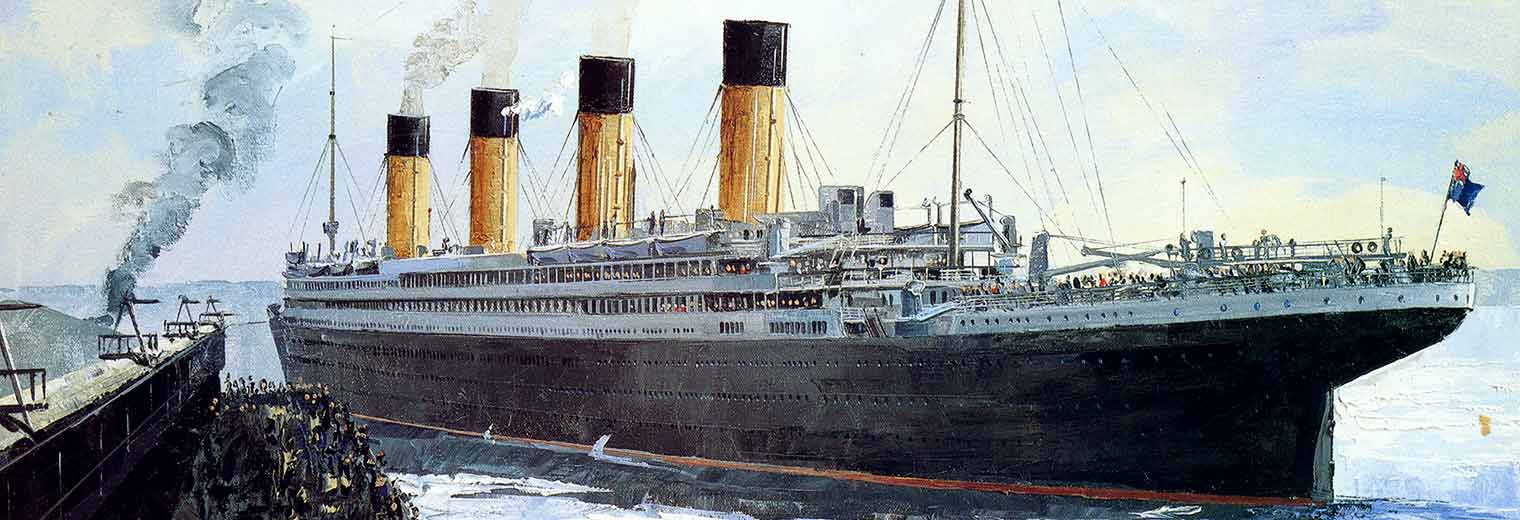
\includegraphics[width=600]{./titanic3.png}
\end{center}
\section*{Afsluiting}
\label{sec:org6444e3d}
Zijn er nog vragen? 
\end{document}